\documentclass[sigplan]{acmart}
\usepackage{subcaption}
\usepackage{caption}
\usepackage{array}
\usepackage{multirow}
\usepackage{placeins}

\renewcommand{\figurename}{Figura}
\renewcommand{\bibname}{Referência}
\AtBeginDocument{
  \providecommand\BibTeX{{
    \normalfont B\kern-0.5em{\scshape i\kern-0.25em b}\kern-0.8em\TeX}}}

\setcopyright{none}
\copyrightyear{}
\acmYear{}
\acmDOI{}

\acmConference[]{Introduction to Research}{December 2021}{Lisbon}
\acmBooktitle{}
\acmPrice{}
\acmISBN{}

\begin{document}

\title{Desenvolvimento de uma Aplicação em Orientação a Objetos}

\author{Pedro Miguel Ferreira Tavares Carrega - 49480}
\affiliation{
 \institution{Estudo Orientado em Engenharia Informática \\ Mestrado em Engenharia Informática \\ Faculdade de Ciências, Universidade de Lisboa}
 }
\email{fc49480@alunos.fc.ul.pt}


\renewcommand{\shortauthors}{Pedro Miguel Ferreira Tavares Carrega - 49480}

\begin{abstract}
Este relatório foi desenvolvido com o propósito de descrever o âmbito do projeto de Engenharia Informática a ser entregue no fim do atual ano letivo e detalhar o trabalho até agora realizado. O projeto está a ser realizado na empresa ARTSOFT, uma empresa com dezenas de anos de experiência a desenvolver soluções de gestão empresarial, em particular o desenvolvimento e comercialização da aplicação ERP ARTSOFT. O propósito do projeto é a integração dos \textit{web services} fornecidos pela Segurança Social e pelos Fundos de Compensação na aplicação ERP ARTSOFT.
\end{abstract}

\keywords{ERP ARTSOFT, OOP, C++, Segurança Social, Fundos de Compensação}

\maketitle

\section{Introdução}

\textit{Enterprise Resource Planning} ARTSOFT é uma aplicação de gestão empresarial que é estruturada em vários módulos, como Gestão Comercial, Contabilidade e Gestão Financeira e Recursos Humanos, permitindo adaptar a solução às necessidades do utilizador. Atualmente, um utilizador da aplicação ERP ARTSOFT que queira submeter o vínculo de um novo trabalhador, tem de utilizar a plataforma online disponibilizada pela Segurança Social; este processo não é eficiente porque obriga o utilizador a submeter duas vezes a mesma informação - primeiro tem de criar a entrada do seu novo empregado na base de dados da aplicação ERP ARTSOFT e de seguida submeter os dados do trabalhador na plataforma da Segurança Social. Num contexto empresarial, este gasto adicional de tempo é muito caro. Foi iniciado um desenvolvimento com o objetivo de oferecer ao cliente a possibilidade de submeter o vínculo de contrato do seu novo trabalhador à Segurança Social diretamente na aplicação ERP ARTSOFT.

Outra funcionalidade oferecida pelo \textit{web service} da Segurança Social é a submissão e atualização da declaração mensal de rendimentos. Atualmente o utilizador pode gerar esta declaração diretamente a partir da aplicação ERP ARTSOFT. Contudo, para submeter ou atualizara mesma tem de utilizar a plataforma online da Segurança Social.

O \textit{web service} dos Fundos de Compensação oferece três diferentes serviços, sendo os três relacionados com o contrato de um trabalhador, ao permitir reportar a admissão de um novo trabalhador, o terminar de contrato de um trabalhador e a atualização dos dados de um contrato. Estas três funcionalidades têm o mesmo objetivo, tal como o \textit{web service} da Segurança Social - poupar tempo ao utilizador.

Com o propósito de integrar os \textit{web services} previamente apresentados, será iniciado um processo de desenvolvimento, começando especificação de requisitos, baseada no estudo da aplicação ERP ARTSOFT e da documentação dos \textit{web services} a integrar; após a aprovação da especificação, e utilizando uma metodologia Agile, serão realizados Sprints quinzenais concluindo com uma bateria de testes funcionais aos serviços integrados.

Neste relatório serão introduzidos e explicados alguns conceitos base para a compreensão do modo de funcionamento dos módulos relevantes da aplicação ERP ARTSOFT e de alguns dos procedimentos internos na empresa. Descreve-se também brevemente a formação realizada em ERP ARTSOFT. É realizada uma análise da documentação dos \textit{web services} a implementar, uma apresentação dos métodos que foram e irão ser utilizados para resolver o problema apresentado e por fim são apresentados os próximos passos a realizar para chegar ao objetivo pretendido.

\section{\textit{Background}} \label{sec:background}

\subsection{Ferramentas Utilizadas}

Nesta secção vão ser apresentadas algumas das ferramentas utilizadas internamente para o desenvolvimento da aplicação ERP ARTSOFT.

\subsubsection{TortoiseSVN}

O TortoiseSVN é um cliente \textit{open source} para a aplicação Apache Subversion, uma aplicação de controlo de versões que corre num servidor centralizado, oferecendo uma interface gráfica, um submenu de contexto no explorador do \textit{windows} e acesso rápido a todos os comandos oferecidos pelo Subversion. Uma arquitetura centralizada oferece várias vantagens em comparação com uma arquitetura distribuída: O repositório encontra-se hospedado num servidor central, retirando a necessidade de clonar o repositório na sua totalidade e permitindo também a atualização somente dos ficheiros locais\cite{subversion}. Ambos estes fatores levam a uma carga inferior da rede. Contudo também implica que se o servidor central se encontrar indisponível, o serviço também está indisponível. Subversion também permite a definição de restrição de acessos e o bloqueio de escrita simultânea de ficheiros, impedido o \textit{merge} de binários.

\subsubsection{Jenkins}

\textit{DevOps} é um conjunto de filosofias e práticas que promovem o desenvolvimento e lançamento de aplicações com uma maior rapidez e qualidade. Duas das práticas mais relevantes são \textit{Continuous Integration} e \textit{Continuous Delivery}. \textit{Continuous Integration} é uma prática que defende que os programadores devem integrar, com regularidade, código desenvolvido para um repositório central sendo este automaticamente compilado e realizados testes sobre o mesmo. Este depois é automaticamente preparado para lançamento, sendo esta a base de \textit{Continuous Delivery}. Com o objetivo de promover estas práticas a empresa ARTSOFT usa a ferramenta Jenkins - um servidor de automação \textit{open source} que corre em \textit{servlet containers} facilitando \textit{Continuous Integration} e \textit{Continuous Delivery} através de \textit{pipelines} para automatizar a compilação de binários através da definição de um conjunto de processos que permitem às pipelines compilar, construir e lançar automaticamente o código produzido.

\subsection{Eventos}

Um evento é um registo interno que é criado na aplicação ERP ARTSOFT sempre que ocorre um acontecimento. Dentro da empresa ARTSOFT é utilizado para efetuar o registo de vários tipos de acontecimentos sendo os mais comuns os eventos de reporte de \textit{bugs} e eventos de \textit{roadmap}. \textit{roadmap} são eventos que envolvem o desenvolvimento de funcionalidades para futuras versões do ERP ARTSOFT. Eventos que reportam \textit{bugs} no funcionamento da aplicação ERP ARTSOFT podem ser criados por reportes internos ou por clientes da aplicação ERP ARTSOFT. Na criação de um evento o utilizador tem obrigatoriamente de fornecer as seguintes informações: o cliente do evento, o tipo de evento e o assunto do evento; adicionalmente é possível adicionar uma mensagem para descrever o evento em mais detalhe e até adicionar imagens. No contexto de um reporte de bug ou \textit{roadmap} é necessário indicar em que módulo do ERP ARTSOFT este evento se enquadra. É possível visualizar esta informação na seguinte imagem:
\FloatBarrier
\begin{figure}[htbp]
	\centerline{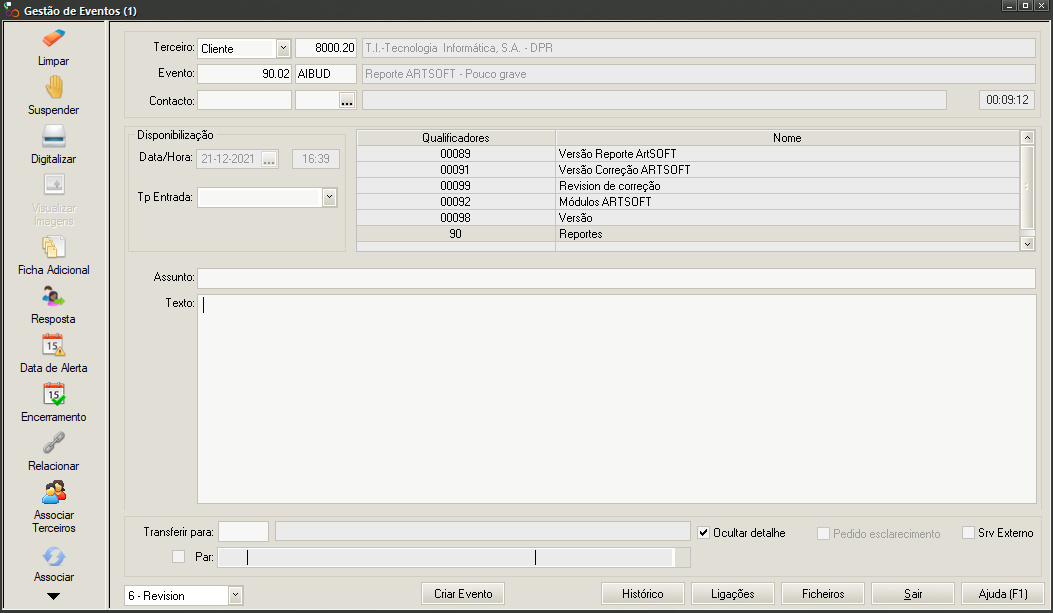
\includegraphics[width=\linewidth]{figures/evento_criacao.png}}
	\caption{Criação de um evento}
	\label{fig1}
\end{figure}
\FloatBarrier
Ao ser criado, um evento de \textit{bug} é enviado para a entrada do Departamento de Programação (DRP); aí é atribuído a um membro da equipa que trabalha para resolver o bug reportado. Ao concluir o seu trabalho, este transfere o evento para a Unidade de Qualidade de Software (UQS) onde a equipa de testes vai testar o evento, confirmando se o mesmo se encontra resolvido. Caso o evento se encontre resolvido é assinalado como tal e é passado para a saída do DPR, senão o evento é passado de volta para o programador responsável pelo evento.

\subsection{Tipo de Entradas}

\subsubsection{Diário}

Um diário é uma coleção de registos de conta que refletem a organização dos documentos contabilísticos da empresa.

\subsubsection{Conta}

Uma conta pode ser representada por uma coleção de documentos, sendo os mesmos associados a um tipo específico de documento.

\subsubsection{Documento}

Em termos simplisticos, um documento representa uma fatu-ra. Dado um tipo de documento o mesmo é automaticamente associado com diário ou uma conta específica.

\subsection{Formação}

Os primeiros meses de trabalho foram dedicados à formação que incluiu os seguintes passos:
\begin{enumerate}
  \item Foram me ensinados os conceitos básicos do funcionamento da aplicação ERP ARTSOFT
  \item O funcionamento das ferramentas utilizadas para o controlo de versões e compilação de binários
  \item O funcionamento de um fluxo de evento
  \item Resolução de um evento de tipo \textit{roadmap} criado somente com o propósito de formação
\end{enumerate}
O evento de tipo \textit{roadmap} que me foi atribuído permitiu que tivesse contacto com tudo que é necessário para efetuar desenvolvimento do ERP ARTSOFT. O objetivo deste evento era oferecer ao utilizador a possibilidade de consultar mais rapidamente e mais facilmente os seus lançamentos contabilísticos, através de uma interface que, dado um de três tipos de entradas - Diário, Documento ou Conta - apresentasse ao utilizador transações associadas à entrada selecionada. Os três tipos de entradas requerem o número da entrada a consultar, sendo possível fornecer diferentes filtros consoante o tipo de entrada seleciona. No caso do Diário é possível limitar ao mês que se pretende consultar enquanto o Documento é possível filtrar pelo tipo de documento. Para este desenvolvimento foi necessário primeiro criar a interface gráfica utilizando as ferramentas fornecidas pelo Visual Studio, que oferece uma interface gráfica para a construção de interfaces; após a criação da interface ligaram-se os controladores aos \textit{inputs} e à tabela; isto permite acesso aos valores inseridos pelo utilizador e a manipulação dos valores da tabela. Uma vez implementado o acesso aos valores introduzidos pelo utilizador na interface, foi necessário implementar o acesso à base de dados de forma a conseguir preencher a tabela e apresentar os resultados ao utilizador. Para isto o ERP ARTSOFT utiliza vários \textit{handlers} para permitir acesso às diferentes bases de dados. Com a nova janela implementada foi utilizado o TortoiseSVN para fazer \textit{commit} do novo código no servidor, utilizando depois o Jenkins para compilar os binários para permitir à equipa de testes testar a nova funcionalidade. Neste caso, sendo formação, o código não foi enviado para o servidor central, nem compilado. Na seguinte imagem é possível visualizar a entrada do evento acima descrito e algumas das mensagens registadas durante o desenvolvimento da funcionalidade:
\FloatBarrier
\begin{figure}[htbp]
	\centerline{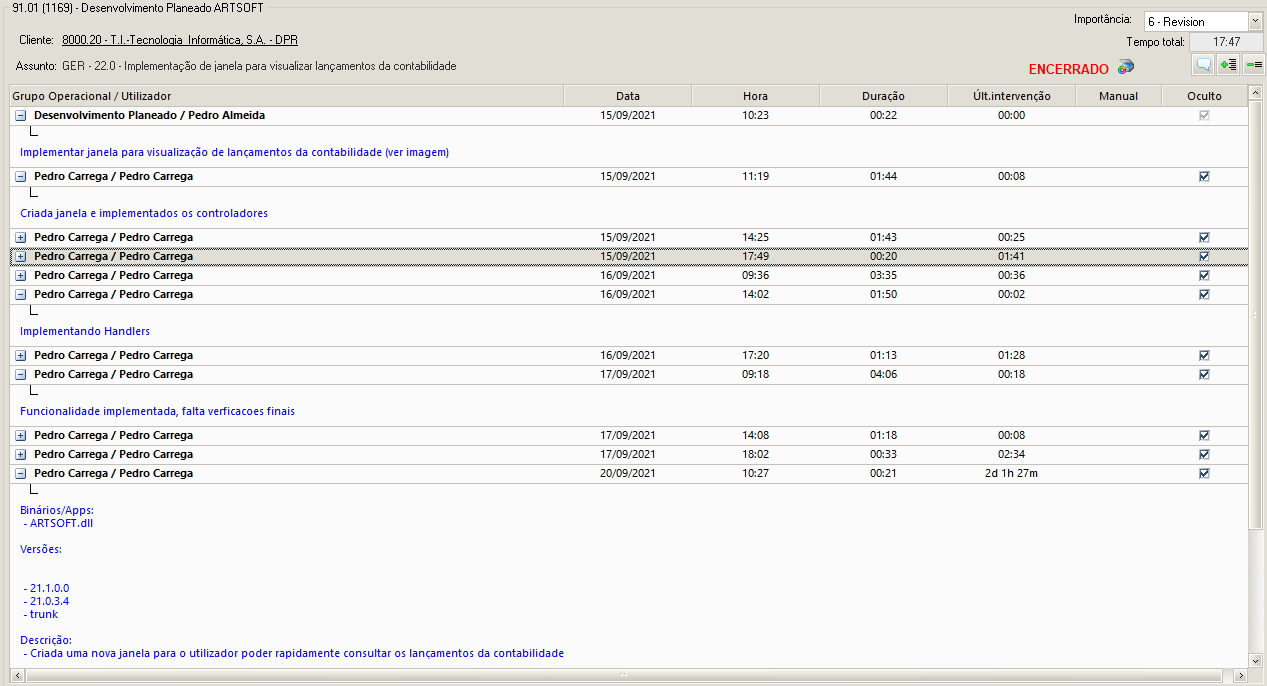
\includegraphics[width=\linewidth]{figures/evento_formacao.png}}
	\caption{Registo do evento de formação}
	\label{fig2}
\end{figure}
\FloatBarrier
A realização deste evento foi ideal para formar um programador a trabalhar na aplicação ERP ARTSOFT pois possibilitou o contacto com a criação de interfaces gráficas e a manipulação das mesmas, como acesso às diferentes bases de dados presentes no ERP ARTSOFT e com algumas das ferramentas já existentes para facilitar o desenvolvimento na aplicação.
\section{Trabalho Relacionado} \label{sec:relatedwork}

%What is the state of the art on the topic you are working? \\

\textit{Web services} é um tema já muito explorado na area de engenharia de \textit{software}. É uma área em constante evolução existindo vários artigos e \textit{papers} que propõe e exploram diferentes metodologias e técnicas de implementação.

%Previous work with same data, similar work with other data, ... \\

%Problems tackled, data science approaches used, pros and cons, ... \\ 

O \textit{paper "Web Services Implementation Methodology for SOA Application"}\cite{SOAA} descreveram que as atuais metodologias utilizadas para o desenvolvimento de aplicações que integram \textit{web services} no seu funcionamento não se revelam suficientes. As principais dificuldades que foram destacadas são - a dificuldade em determinar todos os requisitos da aplicação dado que os requisitos não provém  de uma só fonte; e a implementação no consumo e comunicação do serviço pois diferentes sistemas utilizam diferentes interfaces e métodos de interação. A solução proposta é a integração na metodologia \textit{Agile} as melhores práticas no desenvolvimento de \textit{web services}, contudo os autores não apresentam resultados que suportem a eficacia da sua solução.

\textit{Middlewares} foram criados com o propósito de permitir a comunicação entre diferentes sistemas independentemente da implementação ou \textit{hardware} que utilizem. Contudo, com o aumento da complexidade de \textit{middlewares} o problema para qual foram criados para resolver voltou a surgir, criando uma necessidade de \textit{"middleware for middleware"}\cite{vinoskiMiddleware}. \textit{Web services} tentam resolver este problema mas ao focarem as implementações em usar a SOAP API, os programadores destas soluções estão a ficar aquém do potencial de \textit{web services}. SOAP API não segue um padrão universal, ou seja, diferentes aplicações têm diferentes implementações da mesma. Este é o problema apresentado no artigo de Steve Vinoski\cite{vinoskiIntegration}, que expõem e explica em detalhe um dos problemas que \textit{web services} enfrentam. O autor desenvolve o tema ao apresentar várias soluções, em particular, uma solução em desenvolvimento por uma equipa de engenheiros da \textit{Sun Microsystems} com o nome \textit{Web Services Invocation Framework} (WSIF). Segundo o autor, esta solução resolve vários dos problemas atuais de \textit{web services} mas é longe de ser perfeita sendo exclusiva a soluções que utilizem Java.

\section{Contexto} \label{sec:data}

Para a realização deste desenvolvimento é necessário o estudo extensivo da documentação dos \textit{web services} disponibilizados pela Segurança Social e pelos Fundos de Compensação. Ambos os serviços utilizam HTTPS efetuando os seus pedidos em formato SOAP XML, sendo este um formato muito comum devido à sua versatilidade, usando ambos o mesmo fluxo inicial para efetuar a autenticação com o esquema \textit{HTTP Basic Auth} com a concatenação, codificada em Base64, do nome de utilizador com a \textit{password}; após uma autenticação com sucesso é possível começar a efetuar chamadas ao serviço. Porque seguem o mesmo fluxo - envio de pedido, receção de resposta - analisam-se ao detalhe somente três serviços: um serviço dos Fundos de Compensação e dois serviços da Segurança Social. Na imagem abaixo encontra-se representado o fluxo de qualquer serviço fornecido pelo \textit{web services} da Segurança Social ou Fundos de Compensação.
\FloatBarrier
\begin{figure}[htbp]
	\centerline{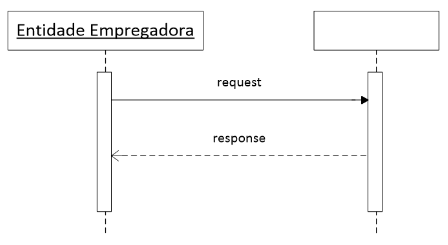
\includegraphics[width=\linewidth]{figures/fluxo_servicos.png}}
	\caption{Fluxo de serviço}
	\label{fig3}
\end{figure}
\FloatBarrier

\subsection{Fundos de Compensação}

O \textit{web service} dos Fundos de Compensação oferece três diferentes serviços, todos relacionados com o contrato do utilizador: o registo de um novo trabalhador nos Fundos de Compensação, o reporte aos Fundos de Compensação da terminação de contrato de um trabalhador e a alteração dos dados de contrato. Neste relatório vamos analisar o serviço de registo de um trabalhador nos Fundos de Compensação. Como mencionado antes, este serviço comunica utilizando HTTPS com os pedidos em formato SOAP XML guardando os dados relevantes ao pedido no corpo da mensagem. No que diz respeito ao pedido de registo de um novo trabalhador, os seguintes parâmetros têm de ser inseridos no corpo da mensagem do pedido a ser enviado:
\begin{itemize}
  \item Número de Identificação de Segurança Social (NISS) do trabalhador;
  \item A modalidade do contrato de trabalho;
  \item A data de início de contrato;
  \item A retribuição base do trabalhador.
\end{itemize}
Existem ainda mais dois parâmetros possíveis de enviar no corpo da mensagem - a data de fim de contrato, sendo este campo obrigatório no caso de um contrato a termo, e as diuturnidades do contrato. O número de identificação de Segurança Social tem de ser um número com onze dígitos e tem de se encontrar válido na Segurança Social; a modalidade do contrato tem de corresponder a um valor pertencente à tabela fornecida na documentação sendo um valor alfabético de A a S; a data de início e fim de contrato tem de obedecer ao formato AAAA-MM-DD sendo a data mínima 2013-10-01; por fim, a retribuição base e diuturnidades são representadas ambas por um número com oito dígitos aonde dois deles representam casas decimais. Depois de submetido o pedido, podem vir dois tipos de respostas; no caso de sucesso, no corpo da mensagem é enviado o número identificador do contrato; no caso de insucesso, no corpo da mensagem é enviado um código de erro cujo valor se encontra presente numa tabela da documentação com uma mensagem de erro descritiva associada.

\subsection{Segurança Social}

No caso do \textit{web service} disponibilizado pela Segurança Social serão implementados somente quatro serviços - a submissão do vínculo de contrato de um trabalhador à Segurança Social, a submissão da declaração mensal de renumerações, a atualização da declaração mensal de renumerações e a consulta do estado de uma declaração mensal de renumerações previamente entregue à Segurança Social. Para o âmbito deste relatório vão ser analisados a submissão do vínculo de contrato do trabalhador e a submissão da declaração mensal de renumerações. No primeiro destes serviços, tal como acontecia no serviço analisado dos Fundos de Compensação, os dados são enviados a partir do corpo da mensagem onde vários deles são obrigatórios:
\begin{itemize}
  \item NISS do trabalhador;
  \item Data de nascimento;
  \item Modalidade de contrato;
  \item Data de início de contrato;
  \item Profissão;
  \item Renumeração base;
  \item Local de trabalho.
\end{itemize}
Além destes existem também os seguintes parâmetros opcionais: a data de fim de contrato, que é obrigatório no caso de o contrato ser a tempo certo ou de muita curta duração, as diuturnidades do contrato, a percentagem, horas e os dias de trabalho no caso de se referir a um contrato a tempo parcial, o motivo de contrato, se o contrato for a termo certo ou incerto, e o NISS do trabalhador a substituir. Muitos dos formatos de dados presentes no serviço dos Fundos de Compensação mantêm-se nos serviços da Segurança Social, ou seja, o NISS é um número com onze dígitos que tem de corresponder a um número válido na Segurança Social, a data de nascimento, início e fim de contrato é uma data com o formato AAAA-MM-DD, a modalidade e motivo de contrato e a profissão são representados por um código alfabético cujos valores se encontram presentes numa tabela fornecida pela documentação do \textit{web service}, a renumeração base e diuturnidades são representados por um número de doze dígitos onde dois deles representam casas decimais, a percentagem, horas, os dias e o local de trabalho são definidos por um número inteiro. O corpo de resposta do serviço de submissão do vínculo do trabalhador é sempre o mesmo independentemente do resultado; é enviado um código de mensagem, códigos definidos por uma tabela presente na documentação, e uma mensagem de erro descritiva caso tenha ocorrido uma falha.

Em relação ao serviço de submissão da declaração mensal de renumerações à Segurança Social, para o envio da declaração mensal de renumerações é obrigatório enviar dois parâmetros no corpo da mensagem - um \textit{array} de bytes que representam o ficheiro a enviar, ficheiro este que se encontra num formato definido pela Segurança Social, e o nome de ficheiro que tem o limite máximo de vinte caracteres e algumas restrições na extensão do ficheiro a ser enviado. Caso a operação tenha tido sucesso, no corpo da mensagem é enviado o código de identificação do ficheiro submetido; em caso de insucesso, no corpo da resposta encontra-se um código de erro e uma mensagem descritiva do erro lançado.

\section{Metodologia} \label{sec:methods}

Como previamente referido, o objetivo deste projeto é a integração dos \textit{web services} providenciados pela Segurança Social e pelos Fundos de Compensação. Estes serviços utilizam HTTPS com as suas mensagens a seguirem o formato SOAP XML para um serviço mais versátil e menos limitado. Vão ser implementados sete diferentes serviços, quatro da Segurança Social e três dos Fundos de Compensação. Da Segurança Social serão implementados o registo do vínculo de contrato de trabalhador e a submissão, alteração e aquisição do estado da declaração mensal de rendimentos. Dos Fundos de Compensação, serão implementados o registo, atualização e conclusão do contrato de um trabalhador. Para integrar estes serviços é necessário primeiro um estudo profundo da documentação disponibilizada cujos resultados serão usados na especificação de requisitos direcionada a este desenvolvimento.

\subsection{Especificação de Requisitos}

Uma especificação de requisitos é um documento cujo objetivo é descrever todos as caracteristicas e comportamentos esperados e desejados de uma aplicação\cite{SRS}. Isto promove o desenvolvimento de um produto de qualidade de superior e que se aproxime o máximo possível das necessidades reais do cliente, para isso a nossa especificação de requisitos vai seguir o seguinte formato:
\begin{enumerate}
  \item Introdução
  \item Sumário
  \item Requisitos
  \item Informação Adicional
  \item Documentos de referência e glossário
  \item Testes
\end{enumerate}
Na introdução são apresentadas as necessidades do cliente de forma a contextualizar o problema, são indicados os módulos que vão ser afetados pelo desenvolvimento e por fim é apresentado o coordenador e programador do projeto, os membros da equipa de teste, o custo estimado e uma estimativa do tempo que irá demorar a desenvolver a solução e a sua margem de erro.

No sumário são resumido em termos técnicos as necessidades do desenvolvimento e as funcionalidades chave a implementar. Na secção dos requisitos são descritos em detalhe, individualmente, os requisitos do desenvolvimento. A estes requisitos é também atribuído um grau de importância, por exemplo, se um requisito criar a necessidade de implementar uma nova interface, isso é explicado em detalhe sendo apresentado um esboço da interface a ser desenvolvida e uma descrição das funcionalidades de todos os botões e campos interativos. No contexto da aplicação ERP ARTSOFT, esta secção contém mais um campo referente a possíveis esboços de relatórios novos a integrar na aplicação. No segmento da informação adicional, como o nome indica, são indicados quaisquer pressupostos e informação adicional que seja relevante para o desenvolvimento. De seguida são apresentados todos os documentos de referência e o glossário, concluindo o documento com a lista de testes aos quais o produto vai ser submetido. No contexto do desenvolvimento a ser realizado neste projeto, foram definidos sete requisitos funcionais:
\begin{enumerate}
  \item Registo do vínculo de trabalhador na Segurança Social;
  \item Submissão da declaração mensal de renumerações à Segurança Social;
  \item Alteração da declaração mensal de renumerações à Segurança Social;
  \item Obtenção de estado de declarações mensais de renumerações previamente entregues à Segurança Social;
  \item Registo da admissão de trabalhador aos Fundos de Compensação;
  \item Alteração dos termos de contrato de um trabalhador aos Fundos de Compensação;
  \item Reportar o fim de contrato de um trabalhador aos Fundos de Compensação.
\end{enumerate}
Aos requisitos 1, 2 e 5 foi atribuída uma importância de grau Crítico, enquanto os restantes requisitos têm uma importância de grau Alto. As funcionalidades referentes aos requisitos 1, 5, 6 e 7 serão acedidas a partir do mesmo ecrã da aplicação, ecrã que já se encontra presente no ERP ARTSOFT. Será adicionado um ícone à toolbar para cada entidade, de modo a que ao clicar nesse botão, apareça um menu \textit{drop down} em que o utilizador clica na funcionalidade que pretende utilizar. Em todos estes requisitos vai aparecer o seguinte ecrã:
\FloatBarrier
\begin{figure}[htbp]
	\centerline{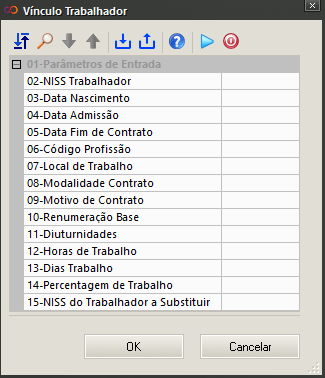
\includegraphics[width=\linewidth]{figures/esboco_interface.png}}
	\caption{Esboço de interface}
	\label{fig4}
\end{figure}
\FloatBarrier
Neste ecrã, o utilizador vai poder validar os dados do trabalhador presentes no sistema. Ao validar os dados, vai-lhe ser apresentada uma mensagem a confirmar o envio do pedido concluindo com a apresentação de uma mensagem ao utilizador a indicar o resultado do pedido. Relativamente aos requisitos 2, 3 e 4 vai ser implementada uma nova interface, com a qual o utilizador pode gerar e visualizar a sua declaração mensal de renumerações e efetuar alterações, se necessário. Além de gerar a declaração mensal de renumerações, o utilizador vai poder selecionar um botão que efetua o envio da declaração mensal de renumerações, depois de ter efetuado a confirmação da ação. No fim, é apresentada uma mensagem a indicar o resultado do pedido. O utilizador também terá a possibilidade de selecionar uma declaração previamente entregue à Segurança Social e efetuar um pedido para determinar o estado da mesma.

\subsection{\textit{Sprints}}

Para este desenvolvimento vai ser utilizada uma metodologia \textit{Agile} que propõe que o desenvolvimento de um projeto deve ser dividido em várias pequenas fases (chamadas \textit{Sprints}) com o objetivo de promover o desenvolvimento incremental da solução. Uma vez começado o projeto inicia-se um ciclo de planeamento, execução e avaliação. O \textit{Sprints} tem um espaço de tempo fixo (entre uma a quatro semanas) onde primeiro é realizada uma reunião para definir os objetivos do atual \textit{Sprints} seguido do desenvolvimento dos objetivos definidos. Após a conclusão do período de tempo estabelecido é efetuada uma avaliação do progresso efetuado durante o \textit{Sprints}, concluindo com uma retrospetiva do que pode ser melhorado para futuros \textit{Sprints} que se repetirão até ao fim do desenvolvimento do projeto. Este projeto será desenvolvido usando a metodologia \textit{Agile} realizando \textit{Sprints} quinzenais.

\subsection{Testes}

Para concluir o desenvolvimento, serão efetuados testes funcionais para verificar que os requisitos se encontram satisfeitos. Estes testes são efetuados de duas maneiras diferentes: testes manuais a serem realizados pelo programador responsável pelo desenvolvimento e por membros da equipa de qualidade de software sendo que estes envolvem o teste do comportamento dos requisitos quer seja em casos de sucesso ou casos de erro; testes automatizados utilizando scripts escritos por membros da equipa de qualidade de software e têm o objetivo de simular a atividade de um utilizador ao utilizar a aplicação. Estes scripts tem o propósito e a capacidade de identificar se os resultados de utilização correspondem ao esperado e se a interface também se comporta como documentado.

\section{Trabalho Futuro} \label{sec:forthcomingwork}

O passo seguinte a realizar no projeto será a realização de uma reunião para apresentar e aprovar a especificação de requisitos. Dada a aprovação, utilizando uma metodologia Agile, serão definidos vários Sprints quinzenais com diferentes objetivos realizando os testes acima descritos no fim de cada Sprint. Estas novas funcionalidades irão ser incluídas na nova versão da aplicação ERP ARTSOFT.

%%
%% The next two lines define the bibliography style to be used, and
%% the bibliography file.
\bibliographystyle{ACM-Reference-Format}
\bibliography{bib/bibliography}
\end{document}
\endinput